\documentclass[arial,english,brazil,oneside]{estilo/estiloifes}

\usepackage[alf]{abntex2cite}
\usepackage[utf8]{inputenc}
\usepackage{lastpage}           % Usado pelo exemplo de ficha catalográfica
\usepackage{microtype}          % para melhorias de justificação
\usepackage{morefloats}         % permite mais floats
\usepackage{listings}
\usepackage{blindtext}          % para gerar texto aleatório (dummy text)
\usepackage{tikz}
\usetikzlibrary[topaths]
\usepackage{mathtools}
\usepackage{float}
\usepackage{setspace}
\usepackage{quoting}
\usepackage{setspace}% http://ctan.org/pkg/{setspace,lipsum}
\usepackage{color, graphicx}
\usepackage[T1]{fontenc}
\usepackage[brazil]{babel}
\usepackage{caption} % Pacote para formatar legendas das figuras e tabelas
\usepackage{url}


%\setlist{parsep=\parskip,leftmargin=1.5cm}
\renewcommand{\baselinestretch}{1.5}
%%% Definição da linguagem padrão do documento (pacote babel) para
%%% definir que certas porções do texto (como o resumo, por exemplo)
%%% estão em uma língua estrangeira, usar as macros
%%% \foreignlanguage{languageB}{Text in another language}
%%% ou
%%% \begin{otherlanguage}{languageB}
%%% ...
%%% \end{otherlanguage}
\selectlanguage{brazil}


%%% Define que todos os códigos fontes construídos com o ambiente
%%% `lstlisting' terão uma borda simples.
\lstset{frame=single}


\newcommand{\ifestex}{\textsf{Ifes$7$}}

\titulo{DESENVOLVIMENTO DE APLICATIVO PARA AUXÍLIO\\DE PAIS E ALUNOS NO CONTEXTO EDUCACIONAL}

\autor{FERNANDO RIBEIRO GARIOLI}
\autorficha{GARIOLI, FERNANDO}

\orientador{DSc. Rafael Vargas Mesquita dos Santos}


\instituicao{INSTITUTO FEDERAL ESPÍRITO SANTO}

\curso{Sistemas de Informação}

\data{2018}

\local{Cachoeiro de Itapemirim}

\preambulo{Trabalho de Conclusão de Curso apresentado à Coordenadoria
  do Curso de Sistemas de Informação do Instituto Federal do Espírito
  Santo, Campus Cachoeiro de Itapemirim, como requisito parcial para a obtenção do
  título de Bacharel em Sistemas de Informação.}

\tipotrabalho{Trabalho de Conclusão de Curso}


\begin{document}



\imprimircapa

\imprimirfolhaderosto*

%\begin{fichacatalografica}
  \vspace*{\fill}
  % Posição vertical
  \begin{center}
    % Minipage Centralizado
    \fbox{
      \begin{minipage}[t]{12.5cm}
        \vspace*{3mm}
        \begin{minipage}[t]{2cm}
          X000x
        \end{minipage}
        \begin{minipage}[t]{10cm}
          \imprimirautorficha.\vspace{2mm}

          \hspace{0.5cm}\imprimirtitulo\ / \imprimirautor. ---
          \imprimirlocal, \imprimirdata.\\ 

          \hspace{0.5cm}\pageref{LastPage} p.:\ il. (algumas color.);
          30 cm.\\ 

          \hspace{0.5cm}\imprimirorientadorRotulo~\imprimirorientador.\\

          \hspace{0.5cm}\imprimirtipotrabalho\ ---
          \imprimirinstituicao, \imprimirdata\\

          \hspace{0.5cm}        
          1. Palavra-chave1.
          2. Palavra-chave2.
          I. Orientador.
          II. Universidade xxx.
          III. Faculdade de xxx.
          IV. Título.
          
          \begin{flushright}
            CDU 00:000:000.0
          \end{flushright}
          \vspace*{1mm}
        \end{minipage}
      \end{minipage}
    }
  \end{center}
\end{fichacatalografica}
%
%%% ====================================================================
%%% Exemplo de construção da folha de aprovação. Depois da
%%% apresentação do trabalho, quando a folha de apresentação real
%%% tiver sido assinada pela banca, a folha real deve ser digitalizada
%%% e o ambiente abaixo deve ser substituído por:
%%% \includepdf{folhadeaprovacao_final.pdf}
\begin{folhadeaprovacao}
  \begin{center}
    {\ABNTEXchapterfont\MakeTextUppercase{\imprimirautor}}\\
    \begin{center}
      \ABNTEXchapterfont\MakeTextUppercase{\imprimirtitulo}\\
    \end{center}
    \hspace{.45\textwidth}
    \begin{minipage}{.5\textwidth}
      {\footnotesize{\imprimirpreambulo}}\\
    \end{minipage}%
  \end{center}
  \vspace{-1cm}%
  \begin{center}
    Aprovado em 26 de Novembro de 2019.\\[15mm]
    \textbf{COMISSÃO EXAMINADORA}\\[5mm]
    \assinatura{\imprimirorientador \\
      Instituto Federal do Espírito Santo - Cachoeiro de Itapemirim \\ Orientador}\vspace{-1cm}
    \assinatura{DSc. Eros Estevão de Moura \\
      Instituto Federal do Espírito Santo - Cachoeiro de Itapemirim}\vspace{-1cm}
    \assinatura{MSc. Flávio Izo\\
      Instituto Federal do Espírito Santo - Cachoeiro de Itapemirim}\vspace{-1cm}
  \end{center}
\end{folhadeaprovacao}
%%%% --------------------------------------------------------------------
%%% Ambiente para escrita da declaração do autor
\begin{declaracaodoautor}

  \vspace*{1.5cm}

  Declaro, para fins de pesquisa acadêmica, didática e
  técnico-científica, que este Trabalho de Conclusão de Curso pode ser
  parcialmente utilizado, desde que se faça referência à fonte e ao
  autor.

  \vspace*{2.5cm}

  \centering

  \imprimirlocal, 20 de Novembro de 2017.

  \vspace*{2.5cm}

  \imprimirautor

  \vspace*{\fill}
  
\end{declaracaodoautor}

%%%% ====================================================================
%%% Ambiente para a escrita da dedicatória.
\begin{dedicatoria}
  \vspace*{\fill}
  \hspace{0.2\textwidth}
  \begin{minipage}{0.8\textwidth}
 Dedico esse trabalho primeiramente a Deus, que até aqui tem me sustentado, e a meu avô, Jefferson Ribeiro Viana.
  \end{minipage}
\end{dedicatoria}
%%%% ====================================================================
%%% Agradecimentos
\begin{agradecimentos}
Agradeço primeiramente a Deus, que até aqui tem me sustentado, me dando força e sabedoria para superar as adversidades.

Em segundo, agradeço a minha família, em especial aos meus pais, Henrique e Rosemere, que sempre me ajudaram quando preciso, e sem os quais este momento também não seria possível.

Aos amigos Gideão e Yuri, que me acompanharam durante toda essa jornada.

Aos professores do Ifes, que sempre desejaram para nós o melhor, minha gratidão por toda a dedicação e conselhos oferecidos. Menção honrosa aos professores Bruno Missi, Eros Moura, Flávio Izo, Everson Borges e João Paulo de Brito, grandes espelhos para mim.

Ao meu orientador e amigo, professor Rafael Vargas, a quem conheço desde os tempos de curso técnico, que sempre me incentivou e inspirou a fazer sempre o melhor.

\end{agradecimentos}
%%%% ====================================================================
%%% Epígrafe
\begin{epigrafe}
  \vspace*{\fill}
  \begin{otherlanguage}{english}
    \begin{flushright}
      \begin{SingleSpace}
      "Clama a mim, e responder-te-ei, e anunciar-te-ei coisas grandes e firmes que não sabes".\\ 
      Jeremias 33:3
      \end{SingleSpace}
    \end{flushright}
  \end{otherlanguage}
\end{epigrafe}
%%% Ambiente para resumo em português
\begin{resumo}
    Este trabalho apresenta uma proposta para o desenvolvimento de um aplicativo \textit{mobile} que visa possibilitar o acesso, em tempo real, a dados acadêmicos de alunos de uma rede municipal de ensino, visando a facilitação da participação e engajamento dos responsáveis na vida acadêmica dos alunos. A aplicação possibilita também, através de um módulo baseado em redes neurais, a classificação de um aluno conforme as áreas de conhecimento definidas na reforma do ensino médio brasileiro. A rede utilizada no módulo desenvolvido obteve uma taxa de 94\% de acerto na classificação dos alunos. O aplicativo proposto foi avaliado por alunos do ensino médio através de formulário de pesquisa, obtendo uma média de aprovação de 88\%.
    
    Palavras-chave: educação, tics, redes neurais.
\end{resumo}
%%% Ambiente para resumo em inglês.
\begin{resumo}[Abstract]
    \begin{otherlanguage}{english}
        This work presents a mobile application development proposal, that aims to provide real-time access to a municipal teaching network academic students data, aimingat facilitating the participation and engagement of those responsible in the studentsacademic life. The application also enables, through a module based on neural networks,the classification of a student according to the areas of knowledge defined in the reformof Brazilian high school. The network used in the developed code obtained a rate of 94\% in the students classification.  The proposed application was evaluated by highschool students through the research form, obtaining an average of 88\% approval.
        
        Keywords: education, tics, neural networks.
    \end{otherlanguage}
\end{resumo}

% \include{listas/listaalgoritmos}
%%% Lista de figuras
\renewcommand{\listfigurename}{Lista de figuras}
\pdfbookmark[0]{\listfigurename}{lof}
\listoffigures*
\cleardoublepage
%%% Lista de tabelas
\pdfbookmark[0]{\listtablename}{lot}
\listoftables*
\cleardoublepage
%%% Lista de quadros
\pdfbookmark[0]{\listadequadrosname}{loq}
\listadequadros*
\cleardoublepage
%%%% Lista de abreviaturas
\begin{abreviaturas}
\item Item 1
\item Item 2
\item Item 3
\item Item 4
\item Item 5

\end{abreviaturas}

%%%% Lista de símbolos
\begin{simbolos}
\simb{$\Gamma$} Letra grega Gama
\simb{$\Lambda$} Lambda
\simb{$\zeta$} Letra grega minúscula zeta
\simb{$\in$} Pertence
\simb{$\top$} Valor lógico máximo dentro de um reticulado regular
  booleano ou quasi-booleano.
\end{simbolos}
\cleardoublepage


%%% Sumário --- Table of Contents
\pdfbookmark[0]{\contentsname}{toc}
\tableofcontents*
\cleardoublepage

\mainmatter

%%% ====================================================================
%%% Início da parte textual do documento.


%%% Configuração do espaçamento entre títulos e texto
\setlength{\afterchapskip}{1.5cm minus \baselineskip}


\chapter{Introdução}
\label{cha:motivacao}
Aplicações educacionais são softwares que promovem o aperfeiçoamento do processo acadêmico de aprendizagem. Tais sistemas proporcionam a seus utilizadores uma perspectiva mais ampla e tangível de informações, trazendo em conjunto funcionalidades suplementares que tornam a relação de aprendizado mais analítica e eficiente. \citeonline{karolcik2015comprehensive} afirmam que o Software Educacional deve ser simples e intuitivo, ao mesmo tempo oferecendo ao usuário um alto nível de comodidade.

Na metodologia de aprendizado, a relação entre escola e família compreende um elemento de vital importância, impactando diretamente na vida acadêmica do aluno. Sua dependência é tal que \citeonline{dessen2007familia} a definem como fundamental no processo de desenvolvimento do indivíduo, impulsionando diretamente seu crescimento intelectual, emocional, físico e social.

O progresso da tecnologia tem condicionado recursos cada vez mais ágeis e interativos, capazes apresentar dados complexos como informação inteligível e comunicativa. Para \citeonline{silva2014novas}, o meio educacional tem reconhecido a importância da tecnologia em seu contexto, e o quão rico é este instrumento para o ensino. \citeonline{silva2016uso} afirmam que estamos diante de um cenário em que a tecnologia digital permite novas formas de ensino, devido a sua riqueza de modelos e conteúdos.

Através disso, podemos destacar a relevância das tecnologias móveis como um elemento de suma importância neste contexto, viabilizando acesso ilimitado e instantâneo à informação. \citeonline{qi2012research} elencam a tamanha aceitação desta tecnologia e o quanto ela se faz presente na vida de milhares de pessoas, substituindo os computadores pessoais como o principal meio de acesso à internet e como forma de trabalho.

O trabalho em questão se insere neste meio, propondo o desenvolvimento de um aplicativo móvel que atue como facilitador na relação entre alunos, pais e escola, objetivando um maior comprometimento das partes no processo de aprendizagem. Dentre suas principais funções podemos destacar:
\begin{itemize}
	\item Disponibilização de dados acadêmicos em tempo real;
	\item Visualização de mensagens da escola e dos professores;
	\item Visualização de tarefas e conteúdos de aulas;
	\item Acompanhamento da frequência e das notas do aluno;
	\item Fornececimento de um ambiente interativo auxiliar para a gestão da vida acadêmica;
\end{itemize}

Neste sentido, propõe-se conjuntamente a utilização de dados dos alunos de para uma análise de padrões, forma a gerar informações auxiliares para alunos e pais. Tal análise se utilizará dos recursos de redes neurais para apontar possíveis fatores capazes de contribuir para o aprendizado do aluno. Deste modo, serão selecionados, com o auxílio de um pedagogo através de coorientação,  parâmetros iniciais básicos, que assistirão ao treinamento da rede proposta, que ocorrerá em seguida.
% ----------------------------------------------------------------------

\chapter{\textbf{Referencial Teórico}} % Este comando é utilizado para criar capítulos
\sloppy % Corrige estouro de linhas

\section{TECNOLOGIA NA EDUCAÇÃO }

O termo ''tecnologia'' diz respeito a muitas outras coisas além das máquinas. O conceito tecnologia engloba a criatividade engenhosa do cérebro humano desde os primórdios da Humanidade. Sua aplicação perpassa pela utilização de diversos recursos naturais, com objetivo de criar ferramentas instrumentais e simbólicas, para transpor barreiras impostas pela natureza até aos testes e aplicação de novas teorias e princípios científicos \cite{kenski2007educaccao}.

A sociedade contemporânea está inserida no momento de constante advento tecnocientífico, e de forma direta e indireta, isto reflete nas práticas pedagógicas escolares. Conforme \citeonline{martins2010gestao}, o educador deve estar sempre atualizado, pois a transformação nos processos tecnológicos e meios de comunicação são permanentes. A presença das TIC (tecnologias de informação e comunicação) na educação é um tema dinâmico e catalisador de transformações no processo ensino-aprendizagem. Estudos demonstram que a condição para o uso com êxito das TIC nas escolas reside, antes de tudo, em saber com utilizá-las e aplicá-las nas atividades curriculares \cite{noeth2004evaluating}. Nesse sentido, a qualificação profissional para o uso das TIC é primordial \cite{david2008padroes}.

De acordo com \citeonline{kenski2007educaccao}, a abordagem didática com integração das TIC no processo ensino-aprendizagem pode alavancar a aprendizagem e o desenvolvimento dos educandos via inserção digital. O grande desafio para escola e educadores, consiste em saber aplicar as TIC como potencializador no sistema educacional, especialmente em seus componentes pedagógicos e processos de ensino-aprendizagem \cite{libaneoorganizacao}.

\section{SISTEMAS DISTRIBUÍDOS}

Na computação moderna vários sistemas computacionais interagem entre si de forma interdependente, sendo a internet o exemplo mais perceptível a ser citado. São várias redes interconectadas e aplicações que fazem uso de tais estruturas para se comunicarem, abrangendo os mais variados domínios. Todas essas estruturas empregam conceitos da tecnologia sistemas distribuídos \cite{puder2011distributed}.\\
\citeonline{tanenbaum2007distributed} descrevem um sistema distribuído como sendo um conjunto de computadores autônomos não obrigatoriamente equivalentes, interligados entre si e compreendidos pelo usuário como um único sistema conexo. Sua compreensão destaca a interdependência e a colaboração entre os computadores como sendo um elemento de suma importância para a existência da arquitetura. A definição proposta por \citeonline[p. 2]{coulouris2005distributed} torna ainda mais precisa através da seguinte definição sobre sistemas distribuídos:

\begin{citacao}
	Definimos um sistema distribuído como aquele no qual os componentes de hardware ou software, localizados em computadores interligados em rede, comunicam-se e coordenam suas ações apenas enviando mensagens entre si.
\end{citacao}

\citeonline{puder2011distributed} destacam vários benefícios dos sistemas distribuídos em comparação com sistemas centralizados, tais como redundância, economia, escalabilidade e tolerância a falhas.

\section{WEB SERVICES}

Considerando as várias utilidades dos sistemas distribuídos, \citeonline{fielding2000} definiu em sua tese de doutorado o REpresentational State Transfer (REST),  um estilo arquitetônico para sistemas hipermídia distribuídos. Tal arquitetura foi desenvolvida com base na disponibilização de recursos, mapeados de forma exclusiva através de URIs (Uniform Resource Identifiers), que são acessadas através de URLs (Uniform Resource Location), funcionando sobre o protocolo HTTP \cite{richardson2008restful}. Em seu trabalho, Fielding destaca seis atribuições básicas que caracterizam o padrão REST, são estas:

\begin{enumerate}
	\item {A aplicação deve utilizar a arquitetura cliente-servidor;}
	\item {Todas as requisições devem ser independentes e isoladas entre si, não havendo nenhum estado de sessão guardado no servidor (Stateless);}
	\item {Requisições já executadas previamente podem ser mantidas em memória para reutilização futura por chamadas equivalentes (Cache);}
	\item {Deve existir uma padronização na manipulação, no mapeamento dos componentes disponibilizados e no formato de troca de dados (Interface Uniforme);}
	\item {O sistema deve ser projetado em camadas, de modo que a interação entre componentes de diferentes camadas seja limitada ao essencial;}
	\item {Código sob demanda, permitindo que applets ou scripts sejam baixados para execução no lado cliente (podendo ser opcional a implementação deste quesito);}
\end{enumerate}

O padrão definido por Fielding se mostra uma alternativa altamente performática em comparação com webservices tradicionais tais como SOAP, principalmente pelo tamanho de mensagens e tempos de resposta menores, tal como afirmam \citeonline{hamad2010} e \citeonline{dudhe2014performance}. A comunidade web e grandes empresas tais como Google e Amazon têm se utilizado dessa tecnologia para construir seus serviços, dado sua simplicidade e escalabilidade \cite{wagh2014hybrid}. REST tem sido amplamente utilizado em conjunto com o JavaScript Object Notation (JSON), uma estrutura de dados simples e leve, em substituição ao formato XML como padrão representativo de troca de dados, sendo suportado pela maioria dos Web Browsers atuais \cite{knutsen2018}.

\begin{figure}[h]
	\caption{Arquitetura de um Web Service RESTful.}
	\caption*{Fonte: \citeonline{thu2015}.}
	\centering % para centralizarmos a figura
	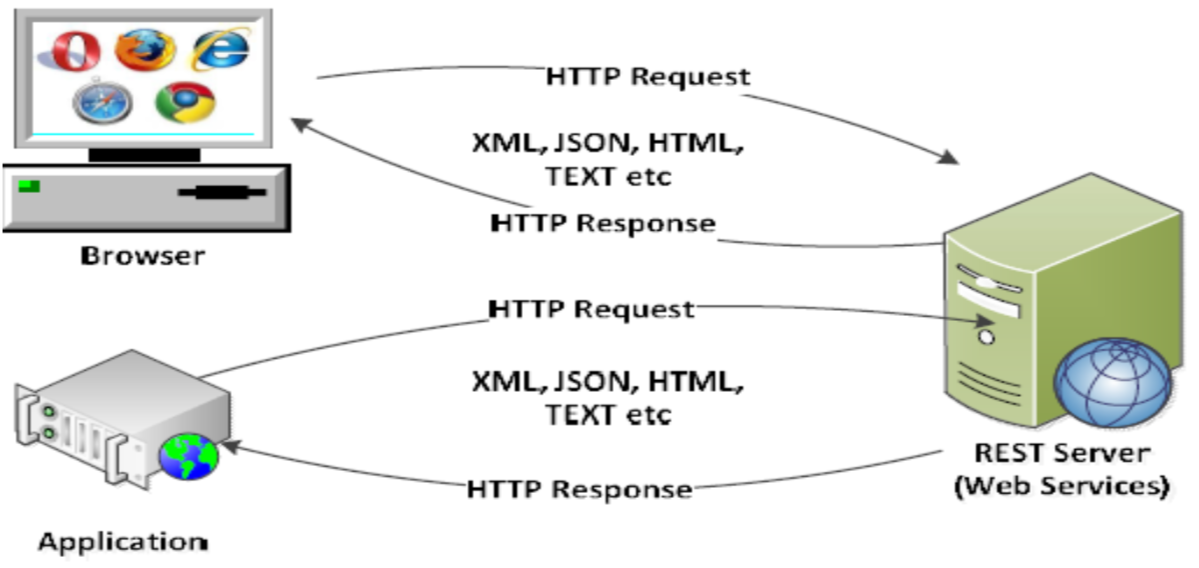
\includegraphics[width=12cm]{resources/webservices.png} % leia abaixo
	\label{figura:webservices}	
\end{figure}

\pagebreak
A figura \ref{figura:webservices} ilustra uma representação básica de um webservice implementado utilizando a arquitetura Rest (RESTful), onde essencialmente são realizadas requisições (HTTP Request) a partir de um determinado cliente (aplicação ou web browser) para um servidor (REST Server), que responde à solicitação com uma resposta (HTTP Response), contendo em seu corpo uma informação padronizada por algum formato representativo de troca de dados (XML, JSON, HTML, TEXT).

\begin{table}[h]
	\captionsetup{justification=centering}
	\centering
	\caption{Métodos HTTP e suas funções correspondentes.}
	\caption*{Fonte: \citeonline{hamad2010}.}
	\label{tabela:metodoshttp}
	\begin{tabular}{r|lr}
		Método HTTP &  Ação\\
		\hline
		GET & Lê um recurso  \\
		POST & Cria um recurso  \\
		PUT & Altera um recurso \\
		DELETE & Deleta um recurso 
	\end{tabular}
\end{table}

Aplicações RESTful utilizam-se dos chamados métodos HTTP para manipulação de dados. A tabela \ref{tabela:metodoshttp} lista os principais métodos e suas respectivas ações, sendo elas leitura, criação, alteração e deleção de dados, respectivamente \cite{pautasso2008restful}.

\section{JSON WEB TOKEN (JWT)}

Quanto à segurança de acesso, web services RESTful podem utilizar mecanismos para garantir que somente usuários autorizados tenham acesso aos recursos. Neste sentido, o padrão JWT (JSON Web Token) \cite{jwt} se mostra uma alternativa concreta para a transmissão de informações confidenciais de autenticação em sistemas stateless \cite{jones2015json}. \citeonline{peyrott2016jwt} descreve tal padrão como um meio simples, compacto e seguro de realizar solicitações, sendo utilizado por uma grande parcela de aplicativos.

\begin{figure}[h]
	\caption{Estrutura básica de um token JWT.}
	\caption*{Fonte: \citeonline{rahmatulloh2018}.}
	\label{figura:jwt}
	\begin{center}
		\textcolor{red}{xxxxxx}.\textcolor{green}{yyyyyyy}.\textcolor{blue}{zzzzzzzz}\\
		\textcolor{red}{header}.\textcolor{green}{payload}.\textcolor{blue}{signature}\\
	\end{center}
\end{figure}

A figura \ref{figura:jwt} ilustra a estrutura básica do JWT, constituída basicamente por uma string de caracteres criptografada denominada Token, dividida em três seções: header, payload e signature.
%\chapter{\textbf{Conclusão}} % Este comando é utilizado para criar capítulos

\section{Análise Geral do Trabalho}
 Seu texto aqui

\section{Trabalhos Futuros}
Seu texto aqui


%%% ====================================================================
%%% Início da parte pós-textual do documento.
\postextual


%%% Referências Bibliográfica

\bibliography{bibliografia/bibliography}

%%%% Início dos apêndices ---------------------------------------------
\apendices


% --------------------------------------------------------------------
\chapter{Titulo}

\begin{enumerate}
    \item Item 1
    \item Item 2
\end{enumerate}

% --------------------------------------------------------------------



%%%% Início dos anexos ------------------------------------------------
\anexos

\partanexos*

\chapter{Exemplo de lombada}

\hspace*{0mm}\fbox{\includegraphics[scale=0.8]{pics/normas-ifes-apendice-d.png}}

\end{document}

